% Section 7.5: Geopolitical alignment and the allied coalition.
% Specification: R/geopolitical_distance/{ideal_points,alignment}.R and scripts/12 (ideal points,
% blocs, dyadic alignment); R/indices/coalition.R and scripts/13 (tiers, routes, EU node weights);
% config/coalition.yml, config/geopolitical_distance.yml. Numbers: paper/results/coalition.json
% (final rerun of 2026-10-12); figures and table: scripts/paper/fig_coalition.R.
\section{Geopolitical alignment and the allied coalition}\label{sec:coalition}

Three parts of the analysis need a coalition: the allied picks of the Strategic Index
(Section~\ref{sec:strategic}), the viewpoint from which the Partnership Strength Index rates partners
(Section~\ref{sec:bilateral}) and the nodes of the network design (Section~\ref{sec:network}). We
derive it by rule from two observable attributes, an economy's alignment in the United Nations
General Assembly and its weight in world supply, rather than fixing it by hand.

\subsection{Ideal points and the U.S.--China axis}\label{subsec:coalition_axis}

Alignment is measured with the ideal points of \citet{bailey2017estimating}, which place every
voting state on one dimension of revealed foreign-policy preference, bridged so that positions are
comparable across sessions. We use the all-votes series of the July 2026 release
\citep[Dataverse V39;][]{voeten2009unga} and average each economy's ideal point $\theta_i$ over
sessions 74 to 78 (2019--2023), which covers the 193 economies that vote in their own right. Each is
placed on the segment between the two anchors,
\begin{equation}\label{eq:coalition_axis}
  s_i \;=\; \min\Bigl\{1,\;\max\Bigl\{0,\;
  \frac{\theta_i-\theta_{\mathrm{CHN}}}{\theta_{\mathrm{USA}}-\theta_{\mathrm{CHN}}}\Bigr\}\Bigr\},
\end{equation}
so that $s_i=0$ is China's position and $s_i=1$ that of the United States
($\theta_{\mathrm{USA}}=2.34$, $\theta_{\mathrm{CHN}}=-1.02$). Seven economies vote further from the
United States than China does and are clamped to zero (Cuba, Iran, Nicaragua, North Korea, Syria,
Venezuela and Zimbabwe). The axis records revealed preferences relative to two anchors, not alliance
or any bilateral relationship.

Following \citet{gopinath2025changing}, blocs are quartiles of the axis: the U.S.-leaning bloc is
the quarter of voting economies closest to the United States ($s_i\geq 0.511$, 49 economies), the
China-leaning bloc the quarter closest to China ($s_i\leq 0.142$, 49), and the 95 in between are
nonaligned. Membership is hard: the bloc indicator $p_i$ is 1 for U.S.-leaning, $\tfrac12$
for nonaligned and 0 for China-leaning economies. Because the United States often votes in small minorities, the distribution is
skewed toward China (median $s=0.22$), and a midpoint rule would call 142 of 193 economies
China-leaning; quartiles keep that bloc to the quarter of the Assembly closest to China. After the
cuts are set, 44 territories inherit their sovereign's bloc and Taiwan, Palestine and Kosovo are
neutral ($p_i=\tfrac12$); these assignments serve only the bilateral indices, and an economy
without its own vote cannot be a core member.

For a pair of economies the dyadic alignment is
\begin{equation}\label{eq:coalition_dyadic}
  A_{ij} \;=\; p_i\,p_j + (1-p_i)(1-p_j),
\end{equation}
which would be the probability that $i$ and $j$ fall on the same side of the divide if $p_i$ were
a probability; with hard blocs it is 1 for the same bloc, 0 for opposite blocs and $\tfrac12$ whenever either is nonaligned. It is a Friendshore
component with weight 2 of 11 (Section~\ref{subsec:friendshore}) and through Friendshore enters the
edge term of the network design. Figure~\ref{fig:coalition_axis} shows the axis by coalition tier.

\begin{figure}[tbp]
  \centering
  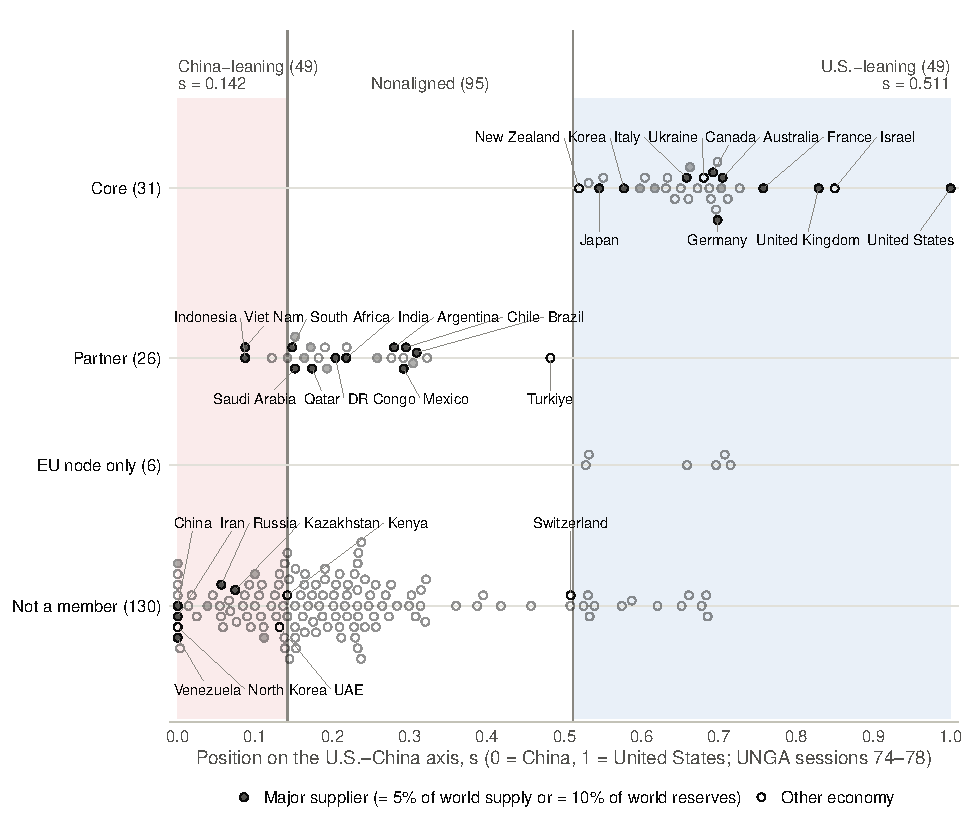
\includegraphics[width=\textwidth]{coalition_axis}
  \caption{Positions on the U.S.--China axis and coalition tiers. Each point is one of the 193
  economies with their own votes in the General Assembly, at $s_i$ of
  equation~\eqref{eq:coalition_axis}: the mean all-votes ideal point of
  \citet{bailey2017estimating} over sessions 74--78 (2019--2023), projected on the segment from China
  ($s=0$) to the United States ($s=1$) and clamped to $[0,1]$. Vertical lines are the quartile cuts
  ($s\leq 0.142$ China-leaning, $s\geq 0.511$ U.S.-leaning; 49, 95 and 49 economies). Rows are the 31
  core members, the 26 partners, the six EU members that enter only through the EU node and the 130
  other voting economies; vertical position within a row carries no information. Filled markers are
  major suppliers (at least 5 percent of world supply in an Upstream or Midstream stage, or at least
  10 percent of world reserves of a headline mineral, fuel or uranium). G20 economies and selected
  other cases are labelled. Source: \texttt{geo\_ideal\_points\_tbl.rds}, \texttt{coalition\_tbl.rds},
  \texttt{major\_supplier\_shares\_tbl.rds}.}
  \label{fig:coalition_axis}
\end{figure}

\subsection{A coalition in two tiers}\label{subsec:coalition_tiers}

The \emph{core} of the coalition $\Coalition$ is the U.S.-leaning bloc restricted to economies with
their own UN votes and a GDP of at least USD 100 billion \citep[2025;][]{worldbank2026wdi}: 31
economies. An economy outside the core is a \emph{partner} if it qualifies by either of two routes.
The agreement route admits members of a U.S. free trade agreement, the Indo-Pacific Economic
Framework (IPEF), the Minerals Security Partnership (MSP), the G7 or NATO with GDP of at least USD
100 billion, whatever their bloc. The supplier route admits, without a GDP floor, any economy that is
not China-leaning and is a major supplier of an Upstream or Midstream stage of a headline
technology: it holds at least 5 percent of world supply in one measure of the stage (exports of the
stage's HS6 basket, fuel or uranium production, mineral mining or refining, or manufacturing
capacity), or at least 10 percent of world reserves of a resource the stage extracts, read from
the reserves tables of the Energy Security pillar \citep{usgs2026mcs,ei2026statistical,oecdnea2026uranium}.
The reserves bar is twice the supply bar because a stock is not yet supply; holders that USGS does
not quantify count as zero. Online Appendix~\ref{oa:coalition} lists the source and year of each
measure.

The rule yields 26 partners (Table~\ref{tab:coalition_composition},
Figure~\ref{fig:coalition_routes}): ten qualify through agreements only, nine as suppliers only and
seven by both routes. Twenty-three are nonaligned and three China-leaning: Indonesia and Viet Nam,
members of IPEF, and Oman, a U.S. free-trade partner. The 57 members account for 73.4 percent of
world GDP (core 57.7, partners 15.7); China accounts for 16.6 percent.

Forty economies pass the supplier test, and every one that is not China-leaning is a member. The
nine China-leaning major suppliers are kept out: China, Russia, Iran, Kazakhstan, Algeria,
Uzbekistan, Venezuela, Myanmar and Zimbabwe, with largest qualifying shares from 94.4 percent of
world graphite refining (China) and 45.1 percent of exports of the uranium basket (Kazakhstan) to 5.1
percent of gas exports (Algeria). Eleven members hold at least 10 percent of a world reserve (Indonesia,
China-leaning, cannot use the supplier route), and for none of the other ten is the reserves leg
decisive. Brazil, in none of the five agreements, holds 23.9 percent of
world graphite reserves, 16.7 percent of manganese, 14.6 percent of rare earths and 11.4 percent of
nickel, and also supplies 18.4 percent of world exports of silicon metal (the Solar Upstream basket).
Among all economies the reserves leg is decisive only for Venezuela, which is kept out.

% Generated by scripts/paper/fig_coalition.R from data/processed/coalition_tbl.rds,
% geo_ideal_points_tbl.rds and major_supplier_shares_tbl.rds
\begin{table}[htbp]
\centering
\begin{threeparttable}
\caption{Composition of the allied coalition}
\label{tab:coalition_composition}
\footnotesize
\begin{tabularx}{\textwidth}{@{}>{\raggedright\arraybackslash}p{0.27\textwidth} r >{\raggedright\arraybackslash}X@{}}
\toprule
Group & $n$ & Economies \\
\midrule
Core: U.S.-leaning bloc, GDP $\geq$ USD 100bn & 31 & United States, Germany, Japan, United Kingdom, France, Italy, Canada, Spain, Korea, Australia, Netherlands, Poland, Belgium, Ireland, Sweden, Israel, Austria, Norway, Denmark, Romania, Czechia, Portugal, Finland, Greece, New Zealand, Hungary, Ukraine, Slovakia, Bulgaria, Croatia, Luxembourg \\
Partners, agreement route only & 10 & T\"urkiye (NATO), Indonesia (IPEF), Singapore (IPEF, U.S. FTA), Thailand (IPEF), Viet Nam (IPEF), Morocco (U.S. FTA), Dominican Rep. (U.S. FTA), Guatemala (U.S. FTA), Oman (U.S. FTA), Costa Rica (U.S. FTA) \\
Partners, supplier route only & 9 & Brazil (Solar Up 18\% [+3]), Saudi Arabia (Oil Up 13\%), Argentina (Batteries Up 6\% [+1]), South Africa (Hydrogen Up 52\% [+3]), Qatar (Gas Up 14\%), Ghana (Batteries Up 10\% [+2]), DR Congo (Batteries Up 66\% [+9]), Gabon (Batteries Up 25\% [+2]), Namibia (Nuclear Up 12\%) \\
Partners, both routes & 7 & India (IPEF, MSP), Mexico (U.S. FTA), Philippines (IPEF), Malaysia (IPEF), Colombia (U.S. FTA), Chile (U.S. FTA), Peru (U.S. FTA) \\
EU members in the EU node only & 6 & Lithuania, Slovenia, Latvia, Estonia, Cyprus, Malta \\
Major suppliers kept out (China-leaning) & 9 & China (Batteries Mid 94\% [+16]), Russia (Hydrogen Up 29\% [+6]), Iran (Gas Up 6\% [+1]), Kazakhstan (Nuclear Up 45\%), Algeria (Gas Up 5\%), Uzbekistan (Nuclear Up 8\%), Venezuela (Oil reserves 18\%), Myanmar (Wind Up 31\% [+1]), Zimbabwe (Batteries Up 9\% [+2]) \\
Reserves holders between 5\% and 10\%, not members & 6 & Madagascar (Graphite 8.7\%), Mozambique (Graphite 8.1\%), Kuwait (Oil 5.9\%), Tanzania (Graphite 5.8\%), Niger (Uranium 5.7\%), New Caledonia (Nickel 5.1\%) \\
Added by the MSP Forum sensitivity & 3 & Kazakhstan, Uzbekistan, Ecuador \\
Hand-picked list of the previous draft: not members & 2 & UAE, Kenya \\
Hand-picked list of the previous draft: members & 21 & 11 in the core, 10 partners \\
\bottomrule
\end{tabularx}
\begin{tablenotes}[flushleft]\footnotesize
\item \emph{Notes:} Economies are ordered by GDP within a group. Core: the U.S.-leaning quartile bloc of the all-votes ideal points of \citet{bailey2017estimating} over UNGA sessions 74--78 (2019--2023), $s\geq 0.511$, with the economy's own UN votes and latest World Bank GDP of at least USD 100bn. Partners (not core): a member of a U.S. free trade agreement, IPEF, the Minerals Security Partnership (MSP), the G7 or NATO with GDP of at least USD 100bn (qualifying agreements in parentheses), or, without a GDP floor, an economy that is not China-leaning and holds at least 5\% of world supply in one measure of an Upstream or Midstream stage of a headline technology (exports of the stage's HS6 basket, fuel or uranium production, mineral mining or refining, or manufacturing capacity) or at least 10\% of world reserves of a headline mineral, fuel or uranium. For the supplier route, the parentheses give the largest qualifying share: the technology--stage cell of a supply measure, or the resource when only reserves qualify, and in brackets the number of further qualifying cells. The six EU members below the GDP floor belong to the coalition only through the EU. The MSP Forum sensitivity admits Forum members by the agreement route. The previous draft's 23 members were fixed by hand.
\end{tablenotes}
\end{threeparttable}
\end{table}


\begin{figure}[tbp]
  \centering
  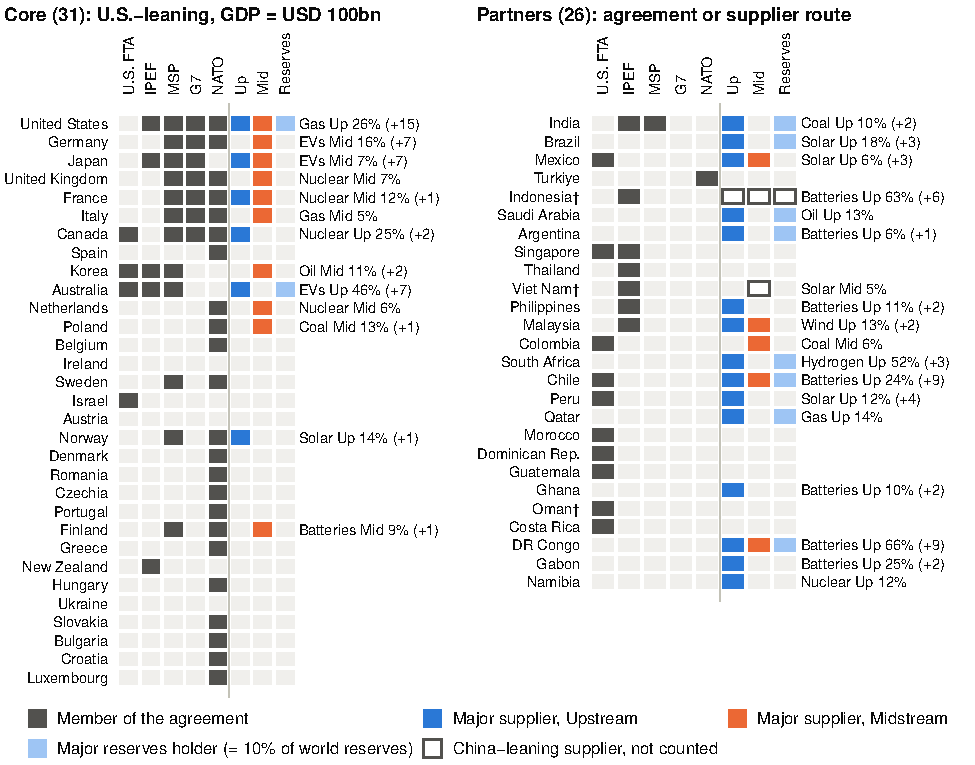
\includegraphics[width=\textwidth]{coalition_routes}
  \caption{Routes into the coalition. Rows are the 31 core members (left) and the 26 partners
  (right), ordered by GDP. Gray tiles mark membership of the five agreements of the agreement route
  (U.S. free trade agreement, IPEF, MSP, G7, NATO). Coloured tiles mark the supplier test: at least
  5 percent of world supply in an Upstream (blue) or Midstream (orange) stage, or at least 10 percent
  of world reserves (light blue). Outlined tiles ($\dagger$) mark economies that pass the test but are
  China-leaning and so cannot use the supplier route; Indonesia and Viet Nam enter through IPEF and
  Oman through its U.S. free trade agreement. The core requires neither route. The text gives the
  largest qualifying share, with the number of further qualifying cells in parentheses. Source:
  \texttt{coalition\_tbl.rds}, \texttt{major\_supplier\_shares\_tbl.rds},
  \texttt{economic\_security\_agreements.csv}.}
  \label{fig:coalition_routes}
\end{figure}

Two economies a reader might expect are not members. Switzerland is nonaligned at $s=0.508$, three
thousandths below the U.S.-leaning cut, belongs to none of the agreements, and its largest supply
share is 1.1 percent; its former supplier route rested on electricity exports, no longer part of
the Electric Grid basket (Section~\ref{sec:data}). Taiwan has no UN vote and is therefore neutral,
appears in no agreement list and has no World Bank GDP; its largest share is 1.5 percent (Solar
Midstream exports), and its semiconductor strength lies outside the energy baskets. Both remain
partners in the bilateral indices but are not network nodes.

The coalition is long in mining and short in processing: its economies mine 81.9 percent of the
world's cobalt and 60.0 percent of its lithium but refine 17.4 and 24.6 percent, and 5.5 percent of
graphite, against China's 75.6, 73.7 and 94.4 percent \citep{iea2026cmdata}; Online
Appendix~\ref{oa:coalition} gives the supply cover by stage.

\subsection{Network nodes and the European Union}\label{subsec:coalition_nodes}

The EU-27 enters the network design as a single node, because the Union conducts a common
commercial policy and its members' supply chains are integrated in a single market. Twenty-one EU
members are core members in their own right; the six below the GDP floor (Cyprus, Estonia, Latvia,
Lithuania, Malta and Slovenia, 1.6 percent of EU GDP) belong to the network only through the node.
The network therefore has 37 nodes representing 63 economies: 11 core nodes (the United States, the
EU, Japan, the United Kingdom, Canada, Korea, Australia, Israel, Norway, New Zealand and Ukraine) and
26 partner nodes. The node's demand enters the design through ranks and is therefore compressed
relative to the EU's share of coalition GDP (Section~\ref{sec:network}).

Members' inputs are aggregated into the node with stage-specific weights
(Figure~\ref{fig:coalition_eu_weights}): production for Coal, Gas and Oil Upstream, exports of the
stage's HS6 basket for 15 cells and GDP for the four Geothermal and Green Hydrogen cells, which have
no basket. The weights are concentrated: Germany carries the largest weight in 11 of the 22 cells,
and France 97.9 percent of the EU's uranium-basket exports although it mines no uranium, trade that
reflects conversion and trading rather than mine output.

\begin{figure}[tbp]
  \centering
  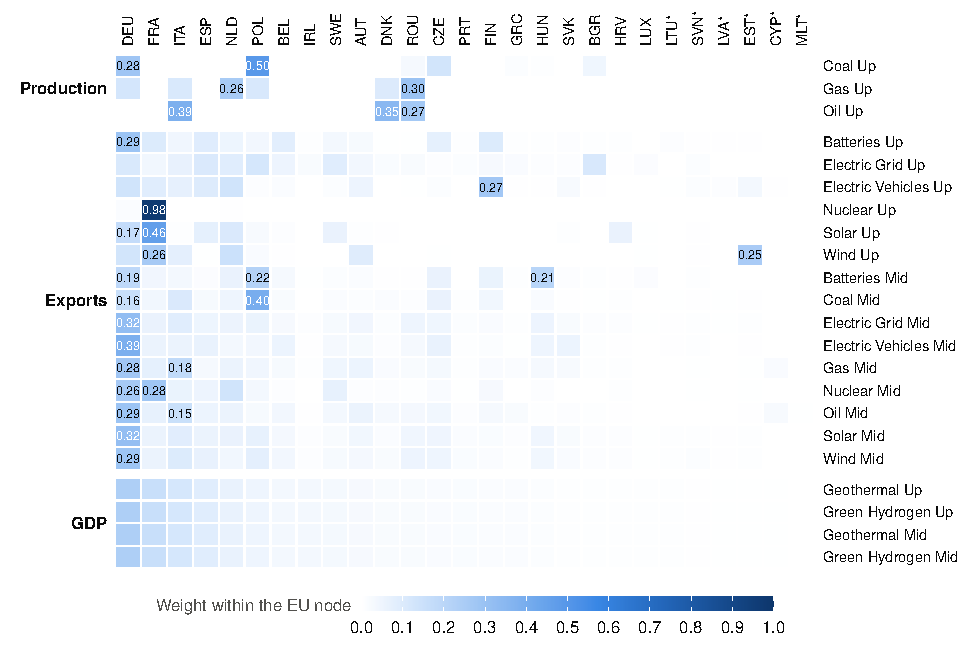
\includegraphics[width=\textwidth]{coalition_eu_weights}
  \caption{Member weights within the EU network node. Columns are the 27 EU members, ordered by GDP;
  an asterisk marks the six members below the GDP floor, which enter the network only through the
  node. Rows are the 22 Upstream and Midstream cells, grouped by the basis of the weights: members'
  production (Energy Institute; 3 cells), members' shares of world exports of the stage's HS6 basket
  (15 cells) or, for the four stages without a basket, GDP shares (Geothermal and Green Hydrogen,
  Upstream and Midstream). Weights in a row sum to one; weights of at least 0.15 under the production
  and export bases are printed. Median Herfindahl index of the weights: 0.34 (production), 0.139
  (exports), 0.117 (GDP). Source: \texttt{eu\_stage\_weights\_tbl.rds}.}
  \label{fig:coalition_eu_weights}
\end{figure}

\subsection{Alignment within the coalition}\label{subsec:coalition_dyadic}

Because the blocs are hard, alignment within the coalition takes a simple form
(Figure~\ref{fig:coalition_alignment_matrix}). Of the 666 pairs of network nodes, 8.7 percent have
$A_{ij}=1$ (pairs of core nodes and pairs among the three China-leaning partners), 86.3 percent have
$A_{ij}=\tfrac12$ because one of the two is a nonaligned partner, and 5.0 percent have $A_{ij}=0$:
each core node paired with Indonesia, Viet Nam or Oman. The alignment component of Friendshore thus
separates core from partner-tier members and penalises the three China-leaning partners as
friendshoring partners of the core, but leaves the ordering of the 23 nonaligned partners to the other components.

\begin{figure}[tbp]
  \centering
  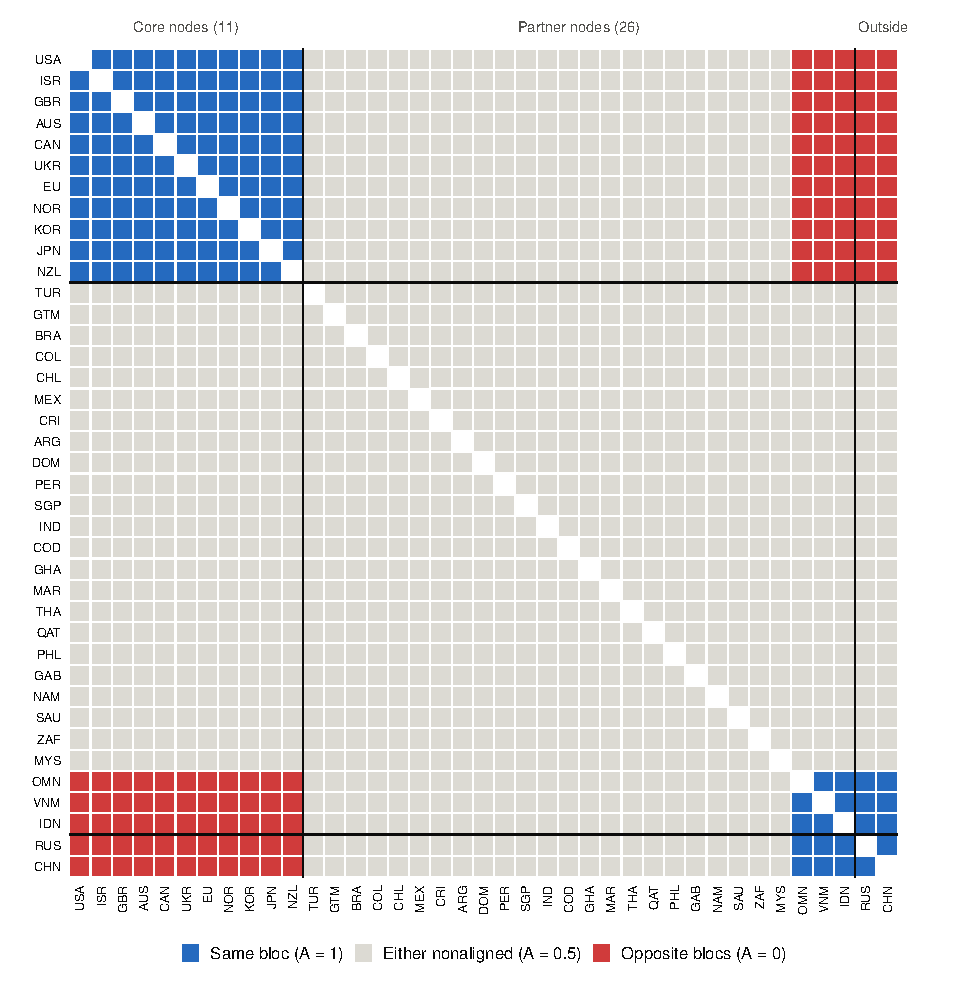
\includegraphics[width=\textwidth]{coalition_alignment_matrix}
  \caption{Dyadic alignment among the network nodes. Each cell is $A_{ij}$ of
  equation~\eqref{eq:coalition_dyadic}: 1 for the same bloc, 0 for opposite blocs and $\tfrac12$
  when either economy is nonaligned. The 37 network nodes, 11 core and 26 partner, are followed by
  Russia and China for reference, ordered by tier and, within a tier, by $s$ (for the EU node, the
  GDP-weighted mean of its members, 0.677; all 27 members are U.S.-leaning). Source:
  \texttt{geo\_alignment\_tbl.rds}, \texttt{allied\_network\_nodes.csv}.}
  \label{fig:coalition_alignment_matrix}
\end{figure}

\subsection{Sensitivity and comparison with the hand-picked list}\label{subsec:coalition_sensitivity}

Two alternative vote series test the axis. With session 78 alone the Spearman correlation of $s$
with the headline is 0.966, 89.1 percent of economies keep their bloc and the coalition keeps 57
members, with three changes at the margin. With the final-passage series over sessions 76--80
(2021--2025) the correlation is 0.965 and the core is unchanged, but the China-leaning cut falls to
0.055: Russia, Kazakhstan and Myanmar leave the China-leaning quartile and would enter as major
suppliers, for 60 members. The core is robust to the vote series; the exclusion of China-leaning
suppliers is the fragile element of the rule. Admitting the MSP Forum as a further agreement adds
Kazakhstan, Uzbekistan and Ecuador.

The derived coalition replaces a list of 23 economies fixed by hand in an earlier version
(Appendix~\ref{app:corrections}). Twenty-one remain; the United Arab Emirates and Kenya, both
China-leaning, in no agreement and without a qualifying share, leave; 36 economies join.

\paragraph{The rule and a functional definition of ``allied''.} The working paper on the Allied
Industrial Base \citep{neis2026allied} argues that ``allied'' should be a functional rather than a
treaty category, with partners assessed on reliability and contractual performance, economic
complementarity, strategic alignment, burden sharing, technology-security requirements and
contribution to system resilience, and with membership varying across sectoral compacts. The derived
coalition implements part of that programme: the axis measures strategic alignment, the supplier
route contribution to world supply and reserves, and the agreement route economic-security ties
with the United States that are already institutionalised. It does not measure reliability, the
rule of law, burden sharing or technology-security requirements, and it defines one coalition for
all 22 stages. The supplier route gives the boundary a sectoral margin (nine partners qualify only
as suppliers of particular stages), but a coalition defined stage by stage, admitting a resource
holder to a minerals compact without admitting it to one on sensitive grid equipment, is left to
future work.
